% Created 2020-09-30 Wed 15:22
% Intended LaTeX compiler: pdflatex
\documentclass[10pt,t]{beamer}
\usepackage[utf8]{inputenc}
\usepackage{graphicx}
\usepackage{grffile}
\usepackage{longtable}
\usepackage{wrapfig}
\usepackage{rotating}
\usepackage{textcomp}
\usepackage{amssymb}
\usepackage{capt-of}
\usepackage{hyperref}
\usetheme{default}
%
\usepackage[font=small,labelfont=bf]{caption} % Required for specifying captions
%
\author{C. L. Hepplewhite}
\date{\today}
\title{\large CHIRP Radiance Corrections/Offsets Connecting AIRS, SNPP, JPSS-1, and IASI}
\subtitle{\footnotesize{AIRS Virtual Science Team Meeting}}
\date{\vspace{0.1in}\footnotesize{October 2020 \vfill}}
\author{C. L. Hepplewhite\inst{1,2}, L. Larrabee Strow\inst{1,2}, and Howard Motteler\inst{2} }
\institute[UMBC]{\inst{1} UMBC Physics Dept. \and \inst{2}UMBC JCET}
\input beamer_setup
\metroset{titleformat title=allcaps}
\setbeamertemplate{frame footer}{UMBC Atmospheric Spectroscopy Lab}
\begin{document}

\maketitle

\begin{frame}{Summary}
\begin{itemize}
  \item What is CHIRP
  \item What are radiance offsets for connecting AIRS, CrIS and IASI.
  \item Data and methods used to derive the radiance offsets.
  \item Results and Discussion.
  \item Integration of offsets into the CHIRP L1C.
    
\end{itemize}

\end{frame}
% -----------------------------------------------------
\begin{frame}{What is CHIRP}

  \begin{itemize}
  \item Climate Hyperspectral InfraRed Product combines AIRS, CrIS, and IASI to provide a homogeneous radiance record, ie
    -  Identical spectral response function
    -  Consistent adiance calibration
  \item CHIRP data are available as level 1 calibrated, geolocated granules.
    (Details are provided in the accompanying presentation by H. Motteler and on-line documentation).
  \item CHIRP V1 uses SNPP CrIS as the radiance standard.
  \item CHIRP spectral resolution equivalent a CrIS with OPD 0.8/0.6/0.4 cm.  
  \item For now, assume radiometric calibration of all sensors is stable.
  \end{itemize}
  

\end{frame}
% -----------------------------------------------------
\begin{frame}{Sensor Radiance Offsets}

  \begin{itemize}
  \item The radiance offset betwen two sensors is the radiometric calibration
    difference observed when they are both measuring the same scene at the same time.
  \item In principle, radiometric calibration offsets could be a function of time and scene radiance (non-linearity).
  \item Existing sensors are already 
  \item Fortunately there is a lot of mission overlap between AIRS, CrIS and IASI
    (more details to follow).
  \item In the first version of CHIRP the radiometric offsets are a static bias (for AIRS and J1 CrIS)
  \item Similar bias offsets exist for IASI and SNPP-CrIS 
  \end{itemize}

\end{frame}

% -----------------------------------------------------
\begin{frame}{Data and Methods}

  \begin{itemize}
    \item Bias derived from (a) SNOs and (b) global random statistical samples.
    \item Available mission overlaps:
      \begin{itemize}
      \item AIRS:NPP from Apr 2012 to present (Dec 2015 at FSR).
      \item AIRS:J1 from Jan 2018 to present.
      \item NPP:J1 from Jan 2018 to present.
      \item AIRS:IASI1 from May 2007 to present.
      \item NPP and J1:IASI1. (Note: SNOs are not available for NPP:J1).
      \end{itemize}
      
    \item Proposed ``recommended'' transition date for parent AIRS to parent CrIS SNPP is 01-Sep-2016.
    \item Switch to JPSS1 for CHIRP proposed for 01-Sep-2018 to avoid the 2019 SNPP CrIS 3-month long mid-wave failure.
  \end{itemize}
\end{frame}

% -----------------------------------------------------
\begin{frame}{Characterisitcs of Overlap Data}

  \begin{itemize}
  \item SNOs have the advantage of being matched pairs of observations, but are spatially less uniformly distributed than global random.
    \begin{itemize}
    \item AIRS:CrIS SNOs are global but weighted to high latitudes,
    \item IASI:CrIS SNOs are restricted to a very narrow latitude band near 70-deg.
    \item SNPP CrIS: J1 CrIS SNOs essentially do not exist!  Use IASI as a transfer standard.
    \end{itemize}
  \end{itemize}
\end{frame}

% -----------------------------------------------------
\begin{frame}{Results 1. AIRS:NPP bias and AIRS modules}

\vspace{-0.1in}
\begin{block}{}
  \begin{center}
    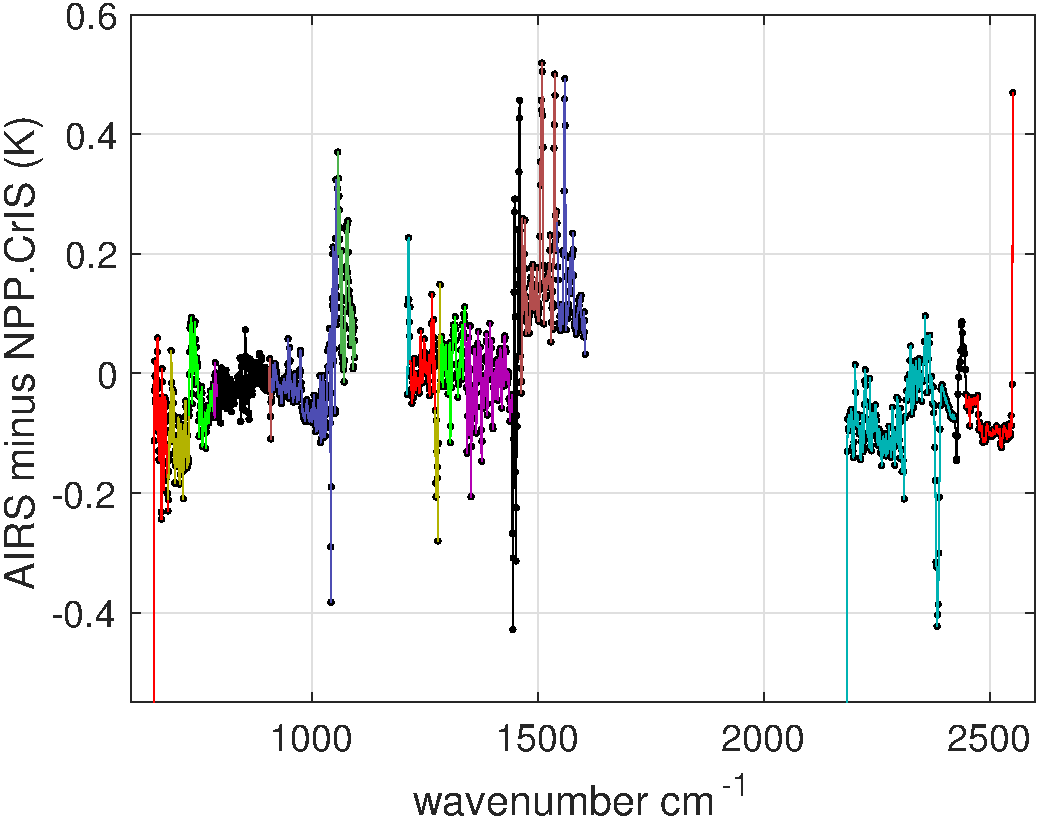
\includegraphics[width=0.6\linewidth]{./Figs/2018_ac1_sno_mean_bias_vs_modules.pdf}
    \captionof{figure}{CHIRP channels. AIRS bias relative to SNPP from global statistics. Showing AIRS module bands.}
  \end{center}
\end{block}
    
\end{frame}

% -----------------------------------------------------
\begin{frame}{Results 2. AIRS:NPP bias with fill and bad channels}

\vspace{-0.1in}
\begin{block}{}
  \begin{center}
    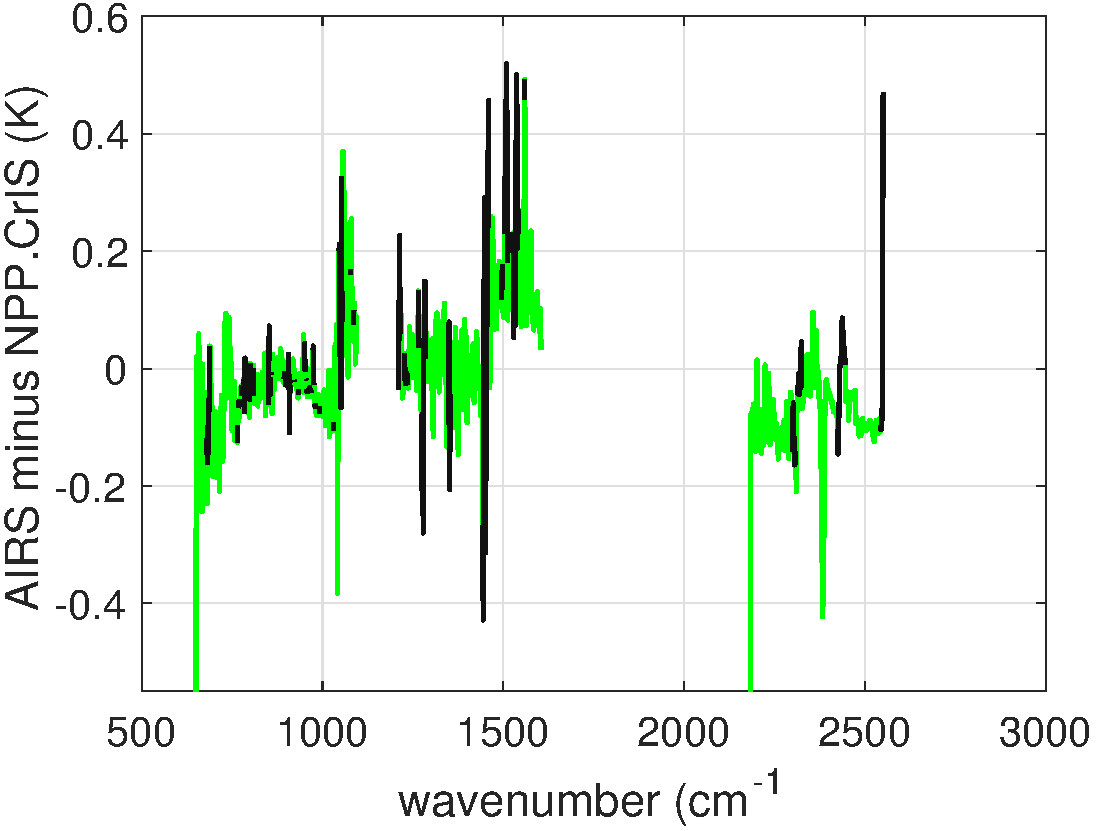
\includegraphics[width=0.6\linewidth]{./Figs/2018_airs_npp_ac1_stats_bias_wbad_fill.pdf}
    \captionof{figure}{CHIRP channels. AIRS bias relative to SNPP from global statistics. Showing parent bad and fill channels (There are 356 such channels.}
  \end{center}
\end{block}
    
\end{frame}

% -----------------------------------------------------
\begin{frame}{Results 3. AIRS:NPP and AIRS:J1 bias}

\vspace{-0.1in}
\begin{block}{}
  \begin{center}
    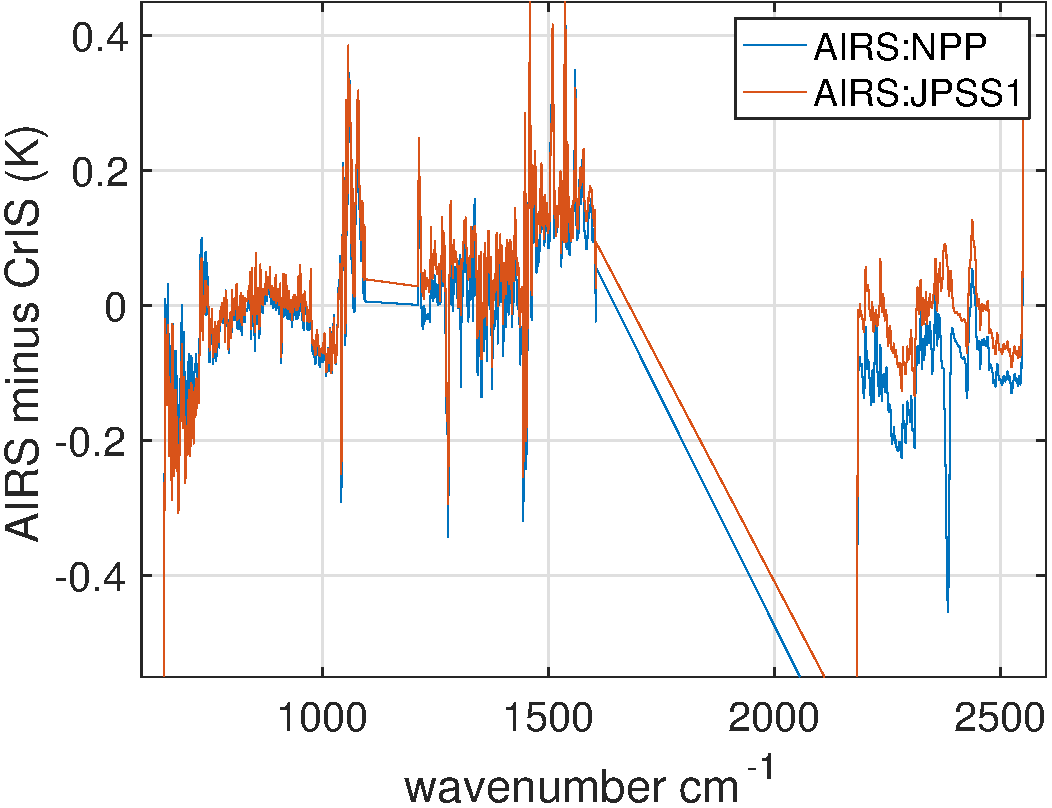
\includegraphics[width=0.6\linewidth]{./Figs/2018d060_2019d059_ac1_ac2_sno_mean_bias.pdf}
    \captionof{figure}{CHIRP channels. AIRS bias relative to SNPP and J1 from SNO. One year of data. Double difference can be used for NPP:J1 bias.}
  \end{center}
\end{block}
    
\end{frame}

% -----------------------------------------------------
\begin{frame}{Results 4. AIRS:NPP bias From Stats and SNOs}

\vspace{-0.1in}
\begin{block}{}
  \begin{center}
    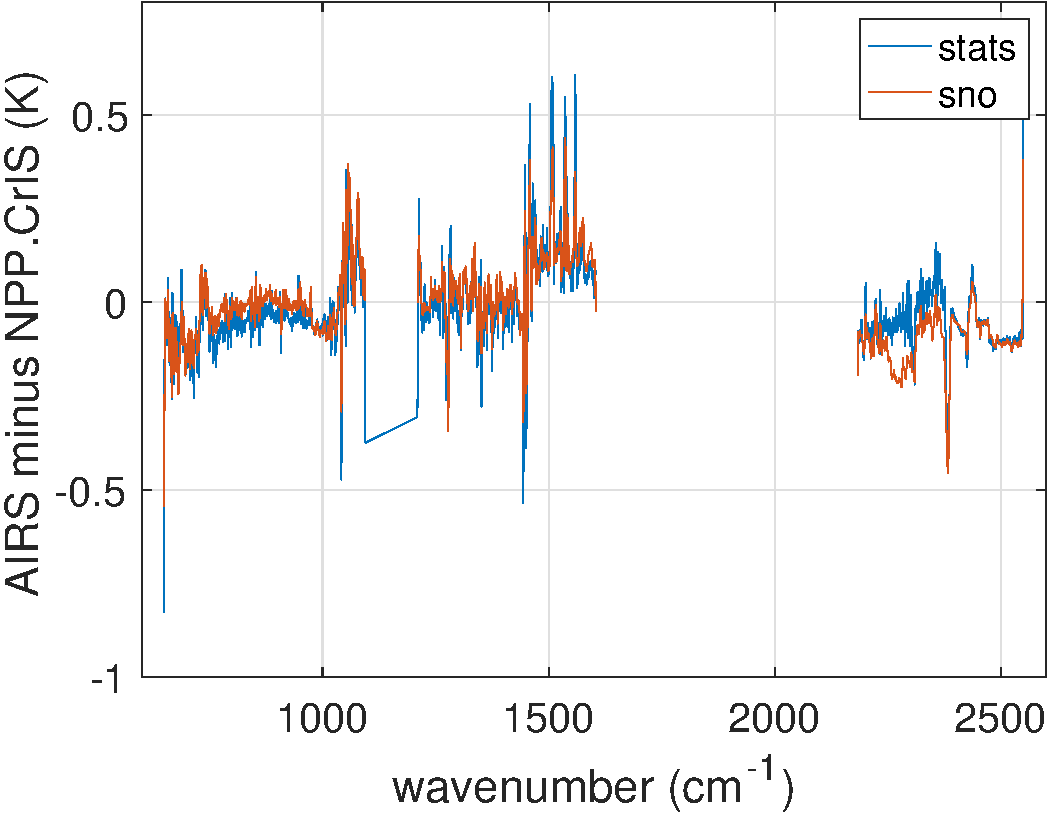
\includegraphics[width=0.6\linewidth]{./Figs/2018d060_2019d059_airs_npp_ac1_bias_stats_sno.pdf}
    \captionof{figure}{CHIRP channels. AIRS bias relative to SNPP from SNO and global stats. showing very close ~30 mK compliance.}
  \end{center}
\end{block}
    
\end{frame}

% -----------------------------------------------------
\begin{frame}{Results 5. J1:NPP bias}

\vspace{-0.1in}
\begin{block}{}
  \begin{center}
    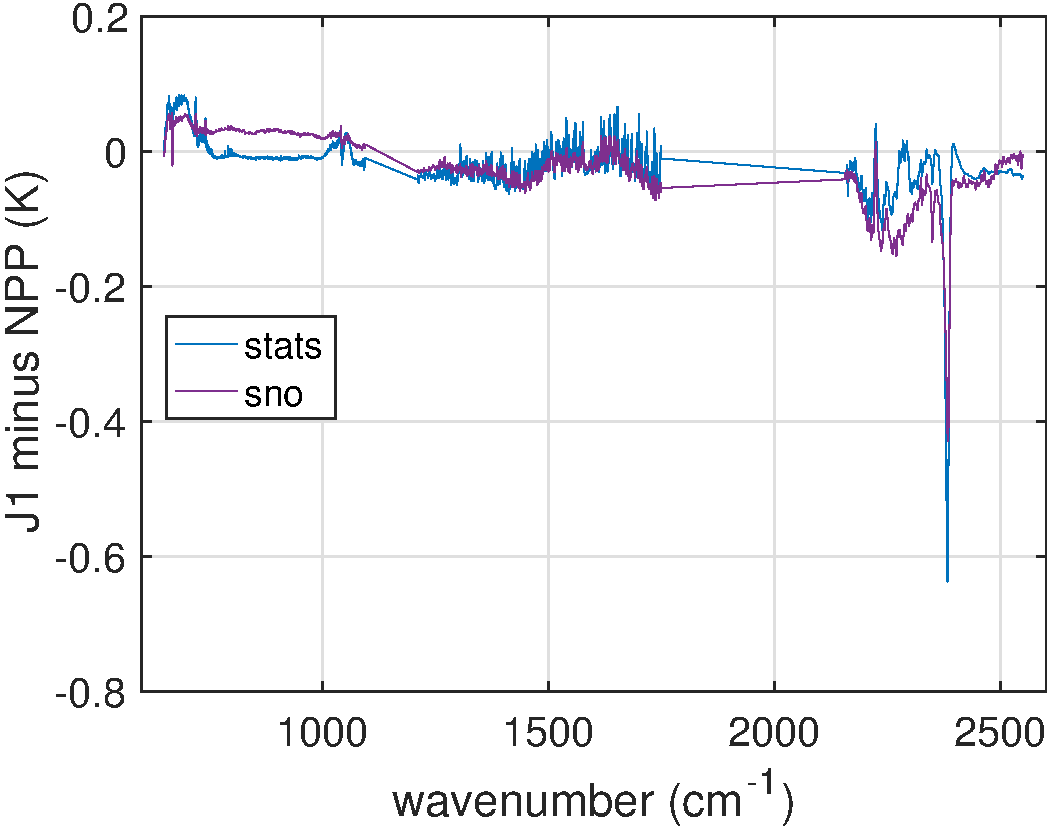
\includegraphics[width=0.6\linewidth]{./Figs/2018_jn_ic1_ic2_stats_sno_bias.pdf}
    \captionof{figure}{CHIRP channels. CrIS bias from JPSS-1 relative to SNPP from SNO using IASI.1 as cross reference and from global random stats.}
  \end{center}
\end{block}
    
\end{frame}

% -----------------------------------------------------
\begin{frame}{Results 6. Bias variation with irradiance.}

  \begin{center}
    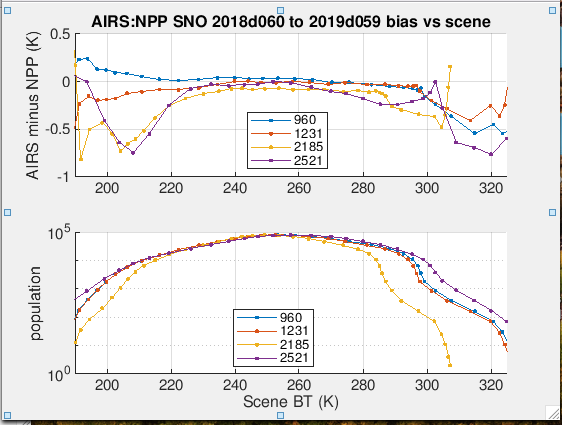
\includegraphics[width=0.6\linewidth]{./Figs/plot1.png}
    \captionof{figure}{Four CHIRP channels. Bias variation with irradiance from SNO.}
  \end{center}

  
\end{frame}

% -----------------------------------------------------
\begin{frame}{Results 7. Sample of bias stability.}

  \begin{center}
    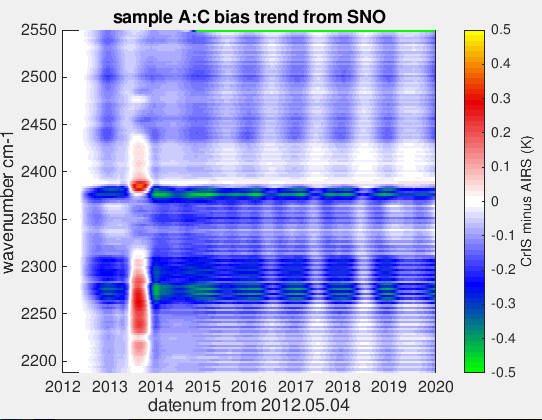
\includegraphics[width=0.6\linewidth]{./Figs/plot6.png}
    \captionof{figure}{CHIRP short wave channels. Bias variation from AIRS:CrIS SNOs. Note residual variation mostly from AIRS solar beta- dependent variation, and 2013 jump to be investigate further.}
  \end{center}
  
  
\end{frame}

% -----------------------------------------------------
\begin{frame}{Summary, Conclusions and Future Work}

  \begin{itemize}
  \item Radiometric offset vectors have been determined to tie CHIRP derived from AIRS to NPP:CrIS and J1:CrIS.
  \item The current CHIRP product includes a single valued vector for every channel.
  \item The bias has been found to be stable over the period of interest, which is 2016 to 2019.
  \item The dependency of bias on irradiance has been investigated, and some examples have been illustrated.
  \item Future work ??
    
  \end{itemize}
  

\end{frame}

% -----------------------------------------------------
%\begin{frame}[label={sec:org409cb32}]{Two}
%\vspace{-0.6in}
%\begin{columns}
%\begin{column}{0.55\columnwidth}
%\begin{block}{}
%\begin{center}
%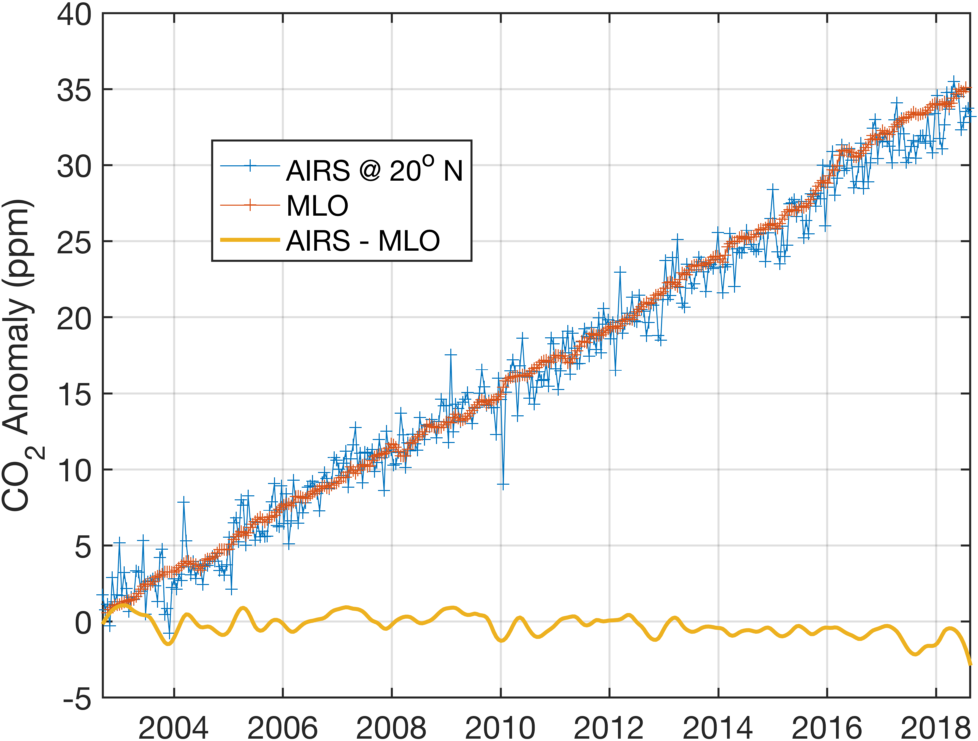
\includegraphics[width=\linewidth]{./Figs/airs_vs_mlo_co2_anom_jun24.png}
%\end{center}
%\end{block}
%\end{column}
%\end{columns}
%\end{frame}
% -----------------------------------------------------

% \begin{center}
% 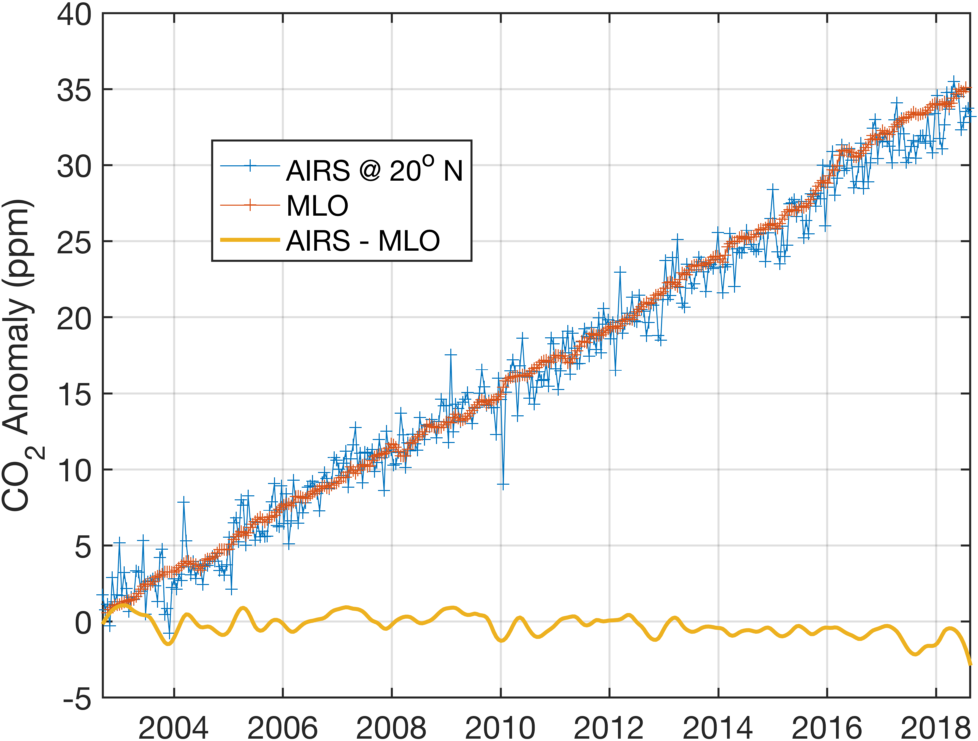
\includegraphics[width=0.8\linewidth]{./Figs/airs_vs_mlo_co2_anom_jun24.png}
% \end{center}

\end{document}
